\documentclass[11pt]{article}

\usepackage[preprint]{acl}
\usepackage{times}
\usepackage{latexsym}
\usepackage[T1]{fontenc}
\usepackage[utf8]{inputenc}
\usepackage{microtype}
\usepackage{inconsolata}
\usepackage{graphicx}
\usepackage{booktabs}
\usepackage{amsmath}
\usepackage{amssymb}
\usepackage{xcolor}
\usepackage{longtable}
\usepackage{url}

\newcommand{\TaskCount}{40}
\newcommand{\ModelCount}{34}
\newcommand{\OpenModelCount}{25}
\newcommand{\ControlModelCount}{5}
\newcommand{\FrontierModelCount}{4}
\newcommand{\RequestCount}{1360}
\newcommand{\SpecificationPassCount}{20}
\newcommand{\SpecificationPassRate}{1.47\%}
\newcommand{\RepairPassCount}{23}
\newcommand{\RepairPassRate}{1.69\%}
\newcommand{\CleanPassCount}{269}
\newcommand{\CleanPassRate}{19.78\%}
\newcommand{\TargetMatchCount}{1}
\newcommand{\TargetMatchRate}{0.07\%}
\newcommand{\PartialOutcomeCount}{679}
\newcommand{\PartialOutcomeRate}{49.9\%}
\newcommand{\SideEffectCount}{3}
\newcommand{\ExpectedEditCount}{202}
\newcommand{\MeanExpectedEdits}{5.05}
\newcommand{\MeanProtectedObjects}{60.55}
\newcommand{\TopModel}{Claude Sonnet 5}
\newcommand{\TopReward}{10.0\%}
\newcommand{\TopRepairPass}{10.0\%}
\newcommand{\TopPreservationPass}{42.5\%}
\newcommand{\TopEditCompletion}{42.7\%}
\newcommand{\TopUCR}{38.0\%}
\newcommand{\TopValidity}{62.5\%}
\newcommand{\FrontierTopModel}{Claude Sonnet 5}
\newcommand{\FrontierTopReward}{10.0\%}
\newcommand{\FrontierTopRepairPass}{10.0\%}
\newcommand{\FrontierTopPreservationPass}{42.5\%}
\newcommand{\FrontierTopEditCompletion}{42.7\%}
\newcommand{\FrontierTopValidity}{62.5\%}
\newcommand{\FrontierTopTruncation}{40.0\%}
\newcommand{\TotalCost}{\$14.88}
\newcommand{\OverallErrorRate}{3.0\%}
\newcommand{\OverallTruncationRate}{37.8\%}
\newcommand{\OverallValidity}{54.2\%}


\title{VectorEditGym: Evaluating Specification-Faithful SVG Repair\\
Under Preservation Constraints}

\author{Yug Aditi Gupta \\
  Theta Labs \\
  \texttt{yug@thetalab.tech}}

\begin{document}
\maketitle

\begin{abstract}
Instruction-based vector editing requires two capabilities: making a requested
change and leaving everything else alone. The second is easy to miss when an
output is judged only as a raster image. We introduce \textbf{VectorEditGym}, a
compact, difficult benchmark of \TaskCount{} SVG repair tasks. Each task pairs a
corrupted SVG program with a human visual instruction, a hidden target program,
\MeanExpectedEdits{} annotated repairs on average, and an average of
\MeanProtectedObjects{} protected objects. Instructions describe visible defects
without exposing element identifiers, coordinates, color codes, or path data.
We define a deterministic binary reward that is one only when the output parses,
implements every annotated repair, and is canonically equivalent to the target;
edit completion and Unintended Change Rate (UCR) diagnose partial outcomes. We
evaluate \ModelCount{} model endpoints (\OpenModelCount{} listed as open-weight,
\ControlModelCount{} inexpensive controls, and \FrontierModelCount{} frontier
closed endpoints) over \RequestCount{} requests.
The strongest endpoint reaches only \TopReward{} binary success, despite
\TopEditCompletion{} requested-edit completion, showing that apparent repair
progress and specification-faithful editing remain substantially different.
All prompts, outputs, scoring code, costs, and per-task reports are released.
\end{abstract}

\section{Introduction}

An instruction such as ``the amber signal has gone dark; fix it and leave the
station alone'' defines both a positive requirement and a large set of negative
requirements. The signal must change, while the train, clock, cables, platform,
and every unrelated program detail must not. A model can produce a plausible
raster while renaming elements, rewriting path data, shifting an unrelated
object, or deleting metadata. These are not cosmetic differences for an SVG:
they alter an executable, structured artifact~\citep{w3csvg2}.

Most generation metrics emphasize final appearance. That is appropriate for
open-ended synthesis, but insufficient for local editing. A repair benchmark
must answer three separate questions: Did the requested objects change? Did
unmentioned objects remain stable? Is the resulting program valid and usable?
VectorEditGym makes all three observable through hidden target SVGs and explicit
protected-object sets.

The benchmark is deliberately small and dense rather than broad and shallow.
Its \TaskCount{} tasks contain \ExpectedEditCount{} annotated repairs across
station, harbor, campsite, market, and larger scenic illustrations. The public
instruction never names a DOM identifier or serialized numeric/path value. Solvers must
interpret the visible scene and edit the source accordingly. Figure~\ref{fig:examples}
shows representative inputs and targets.

Our contributions are:
\begin{enumerate}
  \item a frozen corpus of dense, human-described SVG repairs with explicit
  intended edits and broad preservation surfaces;
  \item a transparent executable evaluator with binary reward, edit completion,
  validity, preservation, and UCR;
  \item a reproducible \ModelCount{}-endpoint evaluation with response
  provenance, token usage, cost, failures, and model-produced SVGs; and
  \item an empirical account of the gap between completing visible repairs and
  preserving the full vector program.
\end{enumerate}

\begin{figure*}[t]
  \centering
  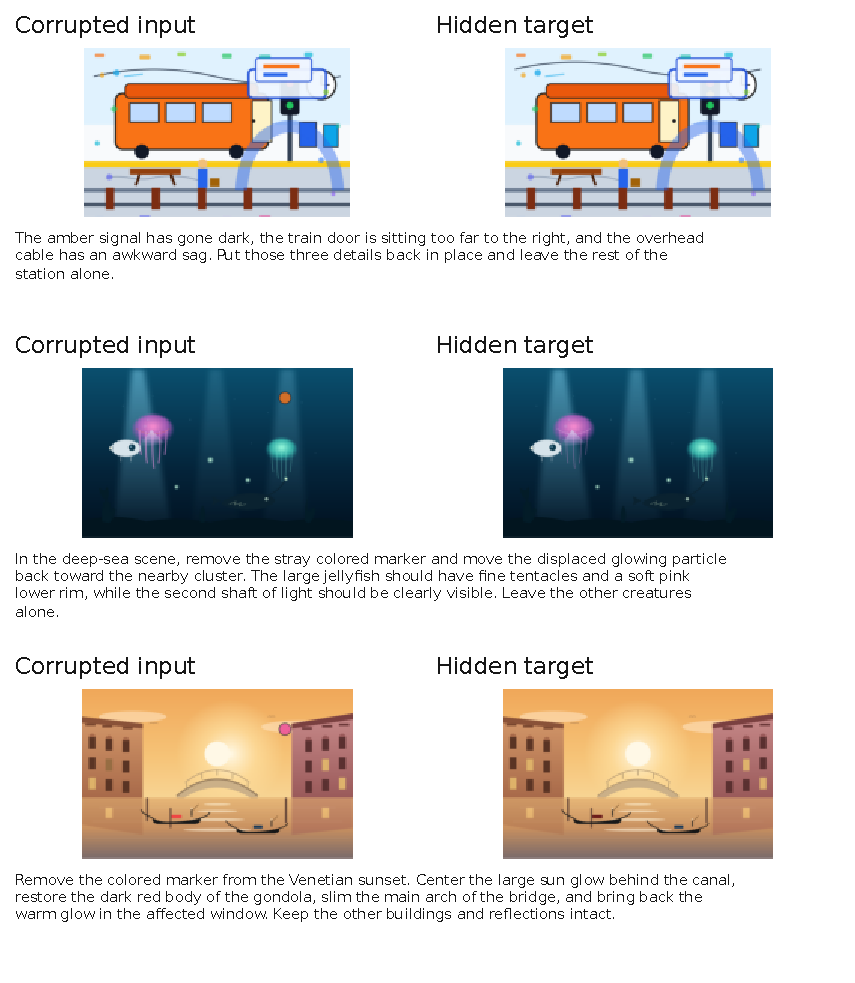
\includegraphics[width=0.98\textwidth]{figures/corpus-examples.pdf}
  \caption{Representative corrupted inputs and hidden targets. Public prompts
  describe visible mistakes in ordinary language without naming source IDs or
  revealing target numeric/path values.}
  \label{fig:examples}
\end{figure*}

\section{Related Work}

\paragraph{Vector generation.}
IconShop generates vector icons from text~\citep{wu2023iconshop}; StarVector
generates SVG code from images and text~\citep{rodriguez2025starvector}; and
LLM4SVG studies complex vector understanding and generation with language
models~\citep{xing2025llm4svg}. These systems establish SVG as a useful meeting
point between visual generation and program synthesis. VectorEditGym focuses on
local repair rather than open-ended generation.

\paragraph{Instruction-based SVG editing.}
SVGEditBench introduced quantitative evaluation for LLM-based SVG editing
\citep{nishina2024svgeditbench}, and SVGEditBench V2 expanded instruction-based
editing evaluation~\citep{nishina2025svgeditbenchv2}. VectorEdits provides a
larger dataset and benchmark for vector-graphics editing
\citep{kuchar2025vectoredits}. Our scope is complementary: we emphasize dense
multi-repair scenes, strict program equivalence after representation
normalization, per-object preservation, and publication of every model output.
We do not claim that a single structural target covers all visually acceptable
edits; instead, we use it to measure specification-faithful repair under an
explicitly strict contract.

\section{Benchmark}
\label{sec:benchmark}

\subsection{Task Format}

Each task is a tuple
\[
  \tau = (x, S_0, S^*, E, U),
\]
where $x$ is a human repair instruction, $S_0$ is the corrupted SVG, $S^*$ is
the hidden target, $E$ is a set of expected object-attribute repairs, and $U$ is
the set of object IDs that must be preserved. The model receives only $(x,S_0)$.
Target source, expected diffs, target-part lists, and preserve lists are excluded
from the prompt and recorded as hidden evaluator inputs.

Instructions were rewritten after task freezing. They describe visible objects
and relations---for example, a moon that drifted down and left or a jellyfish
whose tentacles became too heavy---without SVG IDs, numeric coordinates, hex
colors, path commands, or attribute names. A corpus regression hash covers every
non-instruction task field, ensuring this language-only rewrite did not change
inputs, targets, annotations, or ordering.

\subsection{Composition and Difficulty}

The corpus contains 20 compact but busy scenes derived from four authored scene
templates and 20 larger scenic illustrations. Ten tasks are marked hard and 30
very hard. Tasks require between three and eight repairs, including insertion or
deletion, recoloring, displacement, path restoration, line-weight correction,
and opacity restoration. All unrequested identified parts are protected.

\begin{table}[t]
  \centering
  \small
  \begin{tabular}{lr}
\toprule
Statistic & Value \\
\midrule
Tasks & 40 \\
Annotated repairs & 202 \\
Repairs per task (mean) & 5.05 \\
Protected objects per task (mean) & 60.55 \\
SVG elements per task (mean) & 85.4 \\
Input characters (total) & 294,798 \\
\bottomrule
\end{tabular}

  \caption{Frozen corpus statistics. Element counts include non-rendering SVG
  nodes; protected-object counts refer to identified scene objects.}
  \label{tab:corpus}
\end{table}

\begin{figure}[t]
  \centering
  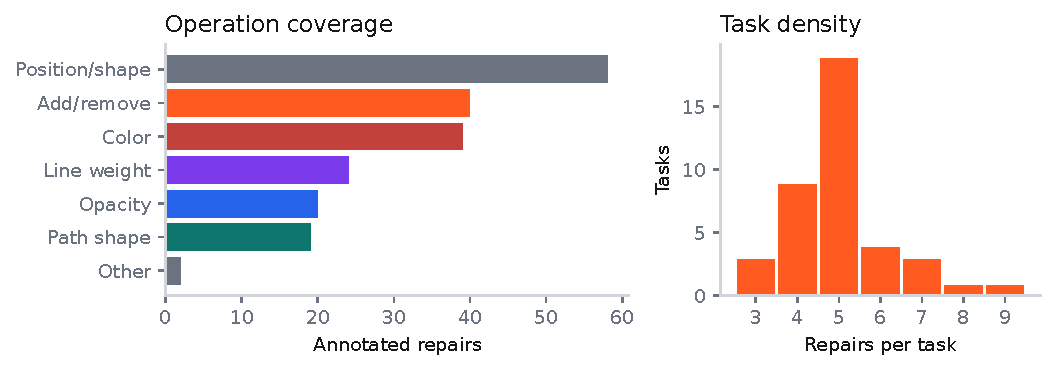
\includegraphics[width=\columnwidth]{figures/task-operations.pdf}
  \caption{Repair operations and per-task edit density.}
  \label{fig:operations}
\end{figure}

\begin{figure}[t]
  \centering
  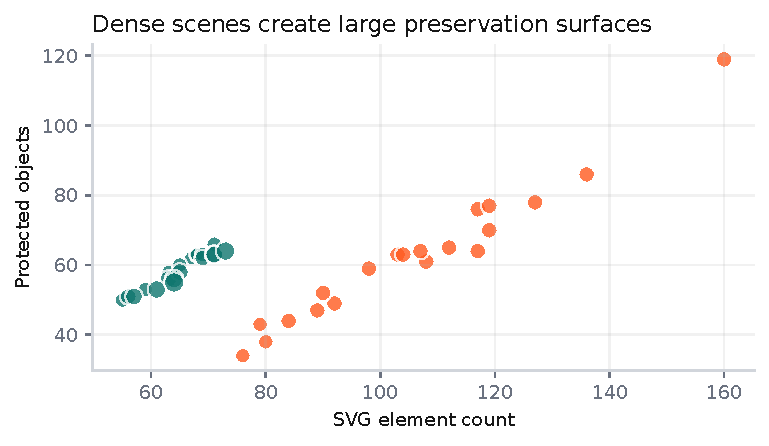
\includegraphics[width=\columnwidth]{figures/task-complexity.pdf}
  \caption{SVG size and preservation surface. Marker area scales with the
  number of requested repairs.}
  \label{fig:complexity}
\end{figure}

\section{Executable Evaluation}
\label{sec:evaluation}

\subsection{Canonical Program Comparison}

Let $C(S)$ parse an SVG and canonicalize representation-only variation. We
discard namespace spelling differences and attribute order, normalize numeric
spellings and separators in paths, points, transforms, and view boxes, and map
common equivalent color spellings (for example, \texttt{white},
\texttt{\#fff}, and \texttt{rgb(255,255,255)}) to one form. Element order,
nesting, IDs, geometry, paint, text, and other program semantics remain strict.
Malformed XML has no canonical form.

The primary reward is binary:
\[
  R(S) = \mathbb{1}\left[C(S)=C(S^*)\right].
\]
Thus a solver receives one point only if every requested repair and every
preservation constraint is satisfied. There is no learned judge, reference
selection heuristic or synthetic reference agent in the public protocol.

\subsection{Diagnostic Metrics}

For expected checks $E$, edit completion is
\[
  \mathrm{Edit}(S)=\frac{1}{|E|}\sum_{e\in E}\mathbb{1}[e(S)=e(S^*)].
\]
For protected objects $U$, preservation and unintended-change rate are
\[
  \begin{aligned}
  \mathrm{Pres}(S)&=\frac{1}{|U|}\sum_{u\in U}\mathbb{1}[C(u_S)=C(u_{S^*})],\\
  \mathrm{UCR}(S)&=1-\mathrm{Pres}(S).
  \end{aligned}
\]
We additionally report parse validity, normalized source exact match, canonical
structural match, provider errors, scheduled elapsed time, tokens, and cost. A provider error
or malformed output receives reward zero. Diagnostic metrics never replace the
binary primary reward.

\section{Model Study}
\label{sec:study}

\subsection{Protocol}

We evaluate \OpenModelCount{} endpoints designated as open-weight in the study
manifest, \ControlModelCount{} inexpensive closed controls, and
\FrontierModelCount{} frontier closed endpoints through the OpenRouter
chat-completions API~\citep{openrouter2026}. These designations record the
endpoint grouping used for analysis and are not an independent license audit.
The exact endpoint IDs appear in Appendix~\ref{sec:full-results}.

Every model receives the same system instruction, human repair request, and
corrupted SVG source. We record one scored outcome per task, omit temperature rather
than imposing a provider-incompatible value, and adapt the output ceiling to
input length (minimum 4,096; maximum 12,000 tokens). The runner retries rate
limits and transient server failures against the same endpoint. It never falls
back to another model; the client permits two transport retries inside each
harness attempt. We record requested and resolved model IDs, response ID,
finish reason, prompt, completion and reasoning tokens when supplied, scheduled
wall-clock elapsed time, and provider-reported cost. Elapsed time begins when a
model--task job is scheduled and therefore includes local concurrency-queue wait;
we expose it for run auditing, not as endpoint latency. Each source cohort uses
a reservation-based budget guard capped at \$25; the completed combined study
cost \TotalCost{}.

\subsection{Uncertainty}

We compute 95\% confidence intervals by resampling the 40 tasks with replacement
10,000 times independently for each model. These intervals quantify task-set
uncertainty only. They do not estimate sampling variance because each
model--task pair has one scored outcome and no repeated decoding. Endpoint tables are ordered by binary reward,
then edit completion, lower UCR, and model name.

\section{Results}
\label{sec:results}

\begin{table*}[t]
  \centering
  \small
  \begin{tabular}{lrrrrrrrr}
\toprule
Model & Full $\uparrow$ & Near $\uparrow$ & Repair $\uparrow$ & Progress $\uparrow$ & Clean $\uparrow$ & UCR $\downarrow$ & Valid $\uparrow$ & Cost \\
\midrule
Claude Sonnet 5 & 15.0 & 2.5 & 15.0 & 50.6 & 42.5 & 0.8 & 62.5 & \$2.032 \\
KAT Coder Air V2.5 & 12.5 & 0.0 & 15.0 & 38.2 & 25.0 & 0.3 & 42.5 & \$0.128 \\
MiniMax M3 & 10.0 & 0.0 & 10.0 & 42.2 & 25.0 & 1.0 & 45.0 & \$0.240 \\
HY 3 & 7.5 & 2.5 & 10.0 & 56.8 & 37.5 & 1.8 & 100.0 & \$0.092 \\
Gemma 4 31B IT & 5.0 & 5.0 & 10.0 & 57.3 & 47.5 & 0.9 & 90.0 & \$0.084 \\
Qwen3.5 397B A17B & 5.0 & 0.0 & 5.0 & 46.7 & 32.5 & 1.4 & 65.0 & \$0.618 \\
DeepSeek V4 Pro & 5.0 & 2.5 & 5.0 & 38.7 & 20.0 & 1.2 & 47.5 & \$0.508 \\
Kimi K2.6 & 5.0 & 5.0 & 5.0 & 29.2 & 15.0 & 0.3 & 25.0 & \$1.077 \\
Qwen3 Coder & 2.5 & 0.0 & 5.0 & 54.7 & 45.0 & 1.4 & 100.0 & \$0.295 \\
Gemini 3.1 Flash Lite & 2.5 & 0.0 & 7.5 & 54.5 & 25.0 & 2.5 & 100.0 & \$0.269 \\
\bottomrule
\end{tabular}

  \caption{Top ten endpoints under binary reward. Reward, edit completion, and
  UCR and validity are percentages; cost is the provider-reported cost for all 40 tasks.
  Full results are in Appendix~\ref{sec:full-results}.}
  \label{tab:main}
\end{table*}

\paragraph{Binary success remains rare.}
Only \BinaryPassCount{} of \RequestCount{} outcomes receive binary reward one
(\BinaryPassRate{}), while \PartialOutcomeCount{} (\PartialOutcomeRate{}) make
at least one annotated repair. The strongest endpoint, \TopModel{}, obtains
\TopReward{} binary reward. Its
edit completion is substantially higher at \TopEditCompletion{}, while its UCR
is \TopUCR{} and its parse validity is \TopValidity{}. The difference is the central benchmark result: models frequently
perform some requested visual work but fail the full repair-and-preserve
contract. Figure~\ref{fig:reward} reports task-bootstrap intervals for every
endpoint.

\paragraph{Frontier endpoints remain subject to the same bottlenecks.}
Within the frontier cohort, \FrontierTopModel{} ranks highest with
\FrontierTopReward{} binary reward and \FrontierTopEditCompletion{} edit
completion. Its parse validity is \FrontierTopValidity{} and its truncation rate
is \FrontierTopTruncation{}. Length-limited outcomes elsewhere in the cohort
remain failures because the protocol requires a complete usable artifact.

\begin{figure*}[t]
  \centering
  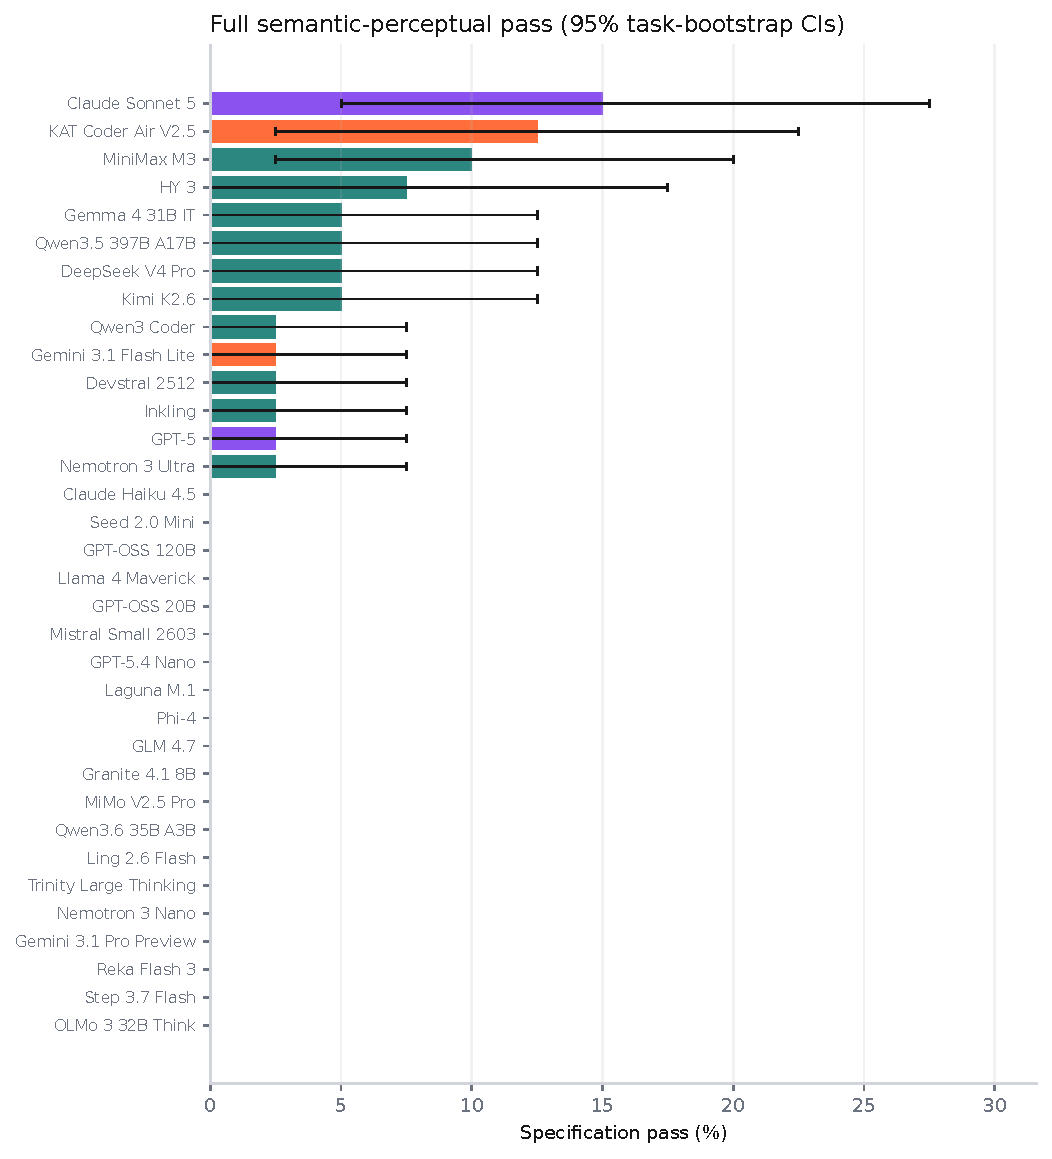
\includegraphics[width=0.84\textwidth]{figures/model-binary-reward.pdf}
  \caption{Binary task success for all endpoints. Orange bars are inexpensive
  controls, teal bars are endpoints listed as open-weight, and purple bars are
  frontier closed endpoints.}
  \label{fig:reward}
\end{figure*}

\paragraph{Repair and preservation are separate axes.}
Figure~\ref{fig:edit-ucr} plots requested-edit completion against UCR. A model can
move right by correcting visible defects while also moving upward by rewriting
protected scene objects. Reporting completion alone would hide this behavior;
reporting only full success would hide useful partial capability.

\begin{figure}[t]
  \centering
  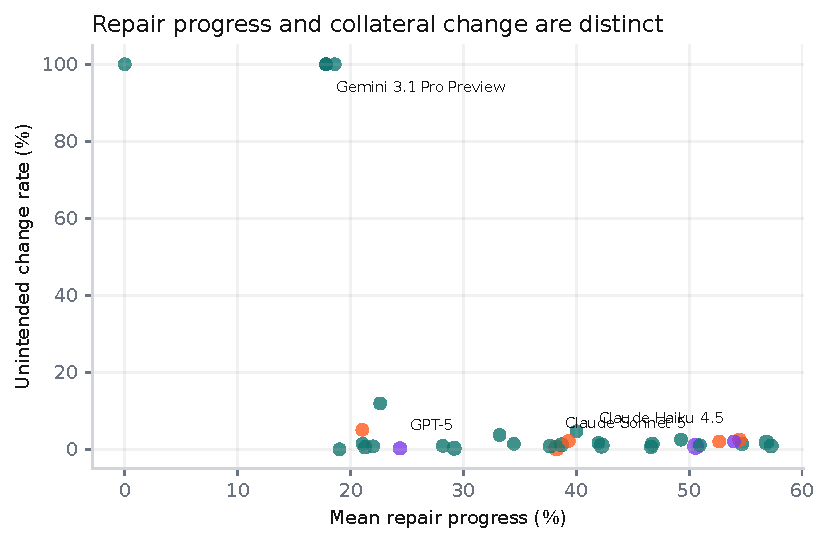
\includegraphics[width=\columnwidth]{figures/edit-completion-vs-ucr.pdf}
  \caption{Requested-edit completion versus unintended-change rate. Marker area
  scales with binary reward. Lower right is preferable.}
  \label{fig:edit-ucr}
\end{figure}

\paragraph{Operation families expose different bottlenecks.}
Figure~\ref{fig:heatmap} decomposes the expected checks. Simple color or
add/remove corrections need not predict path-shape or position restoration,
especially because the prompt gives visual descriptions instead of literal DOM
values. This decomposition also distinguishes an endpoint that attempted an edit
but selected the wrong source element from one that returned an invalid or
unchanged document.

\begin{figure*}[t]
  \centering
  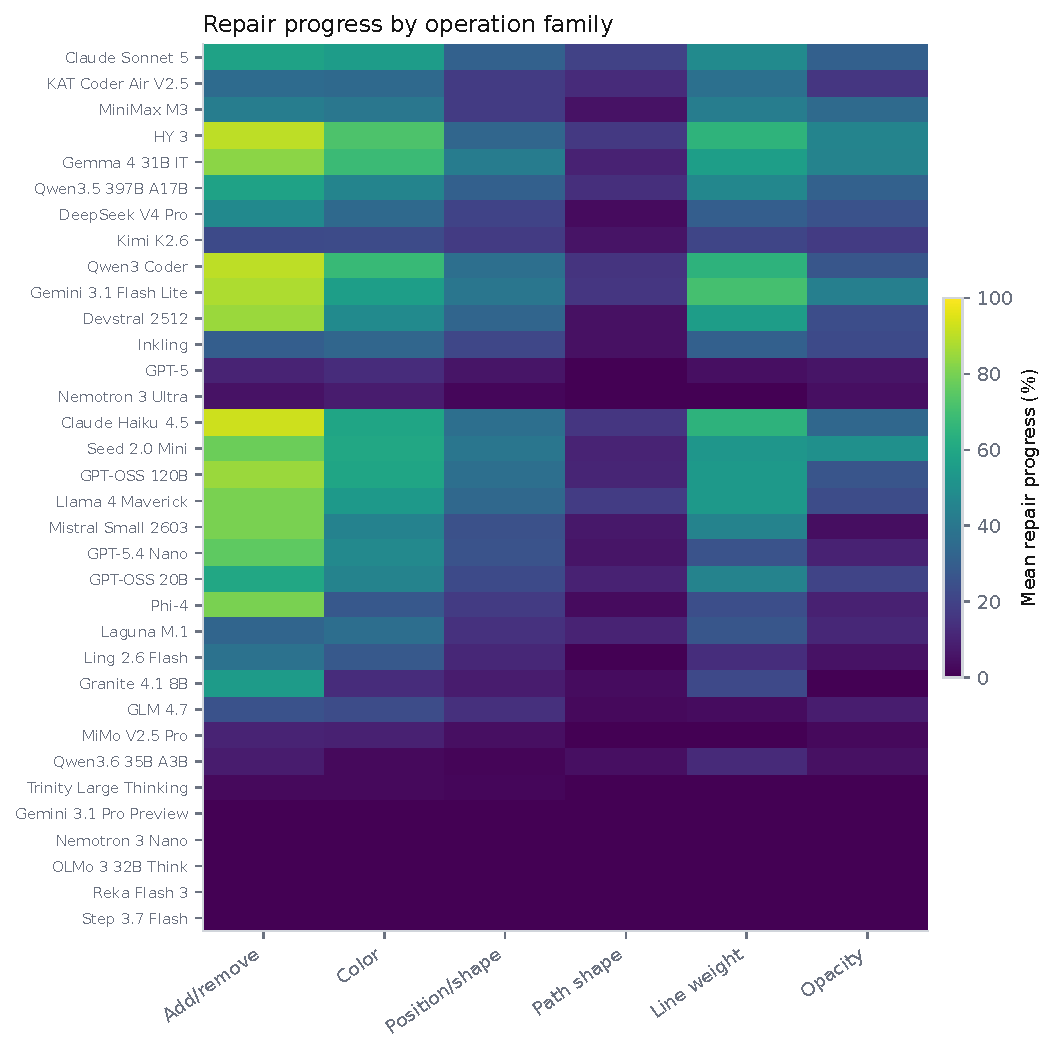
\includegraphics[width=0.88\textwidth]{figures/operation-heatmap.pdf}
  \caption{Expected-edit check success by operation family. Rows follow overall
  binary-reward rank.}
  \label{fig:heatmap}
\end{figure*}

\paragraph{Cost is not a sufficient capability proxy.}
The run spans inexpensive small endpoints and larger reasoning or coding models.
Figure~\ref{fig:pareto} shows edit completion against total 40-task cost. It is a
descriptive endpoint comparison rather than a hardware-efficiency claim:
OpenRouter pricing and routing can change, and the study uses one scored outcome
per task.

\begin{figure}[t]
  \centering
  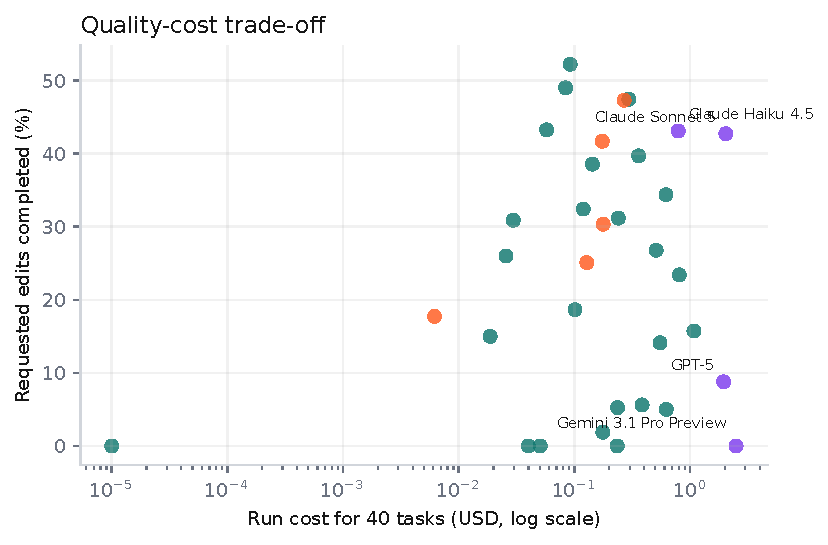
\includegraphics[width=\columnwidth]{figures/quality-cost-pareto.pdf}
  \caption{Edit completion versus provider-reported run cost.}
  \label{fig:pareto}
\end{figure}

\section{Error Analysis}

\paragraph{Literal partial repair.}
Models often identify an obvious semantic defect, such as a signal with the wrong
color, while leaving a displaced object or malformed curve unresolved. These
outputs earn partial edit-completion credit but binary reward zero.

\paragraph{Global rewrites.}
Some responses regenerate or reformat substantial portions of the SVG. Canonical
normalization accepts harmless formatting, but changed paths, reordered scene
objects, renamed IDs, or missing definitions count as program changes. Protected
object checks identify which named scene components drifted; document-level
checks catch anonymous definitions and root attributes.

\paragraph{Ambiguous visual recovery.}
Human prompts intentionally omit exact coordinates and path commands. A model may
make a visually reasonable adjustment that differs from the frozen target. The
strict reward records that as failure. This is useful for evaluating exact repair
of structured assets but should not be interpreted as a complete perceptual
quality judgment.

\paragraph{Provider and truncation failures.}
Only \OverallValidity{} of scored outcomes contain parseable SVG. The harness
preserves raw malformed output, API errors, and finish reasons in the released
records. Transient failures are retried only against the requested endpoint;
persistent failures remain zero-scored observations. The aggregate provider
error rate is \OverallErrorRate{}, and \OverallTruncationRate{} of all outcomes
end at the provider's output-length limit; parse failure is measured separately.

\section{Limitations and Artifact Risks}

VectorEditGym has only \TaskCount{} tasks and should be treated as a focused
stress test, not a comprehensive measure of visual editing. Public targets make
future contamination possible. The single-target structural reward can reject
visually or semantically acceptable alternatives, and our basic color
canonicalization is not a complete CSS equivalence engine. Conversely, canonical
tree equality does not test downstream animation, scripting, accessibility, or
editor-specific behavior.

The evaluation uses one scored outcome per model--task pair and therefore cannot
characterize sampling stability. OpenRouter can change prices, routing, model versions, and
availability; requested and resolved IDs are published to make this visible.
The ``open-weight'' grouping is manifest metadata, not a legal determination.

Twenty scenic source files in the frozen corpus lack recoverable per-file
provenance metadata. We do not claim original authorship of those illustrations.
They are retained to preserve the evaluated task set, marked as provenance
pending in the artifact, and should be treated as research-only until provenance
is resolved. This limits redistribution confidence and is a material artifact
risk.

Finally, the benchmark evaluates text-and-source editing rather than multimodal
screen interaction. Models see SVG code and a visual description, but not a
raster preview or interactive editor. Performance therefore combines scene
reasoning, source localization, and code generation under one protocol.

\section{Conclusion}

VectorEditGym isolates a practical requirement for editing agents: requested
change is not enough; preservation is part of the specification. Human visual
instructions make the task less like copying a patch, while executable SVG
targets make every decision auditable. Across \ModelCount{} endpoints, partial
repair is much more common than exact repair-and-preserve success. The released
outputs and diff reports make that gap inspectable at the object and source level
and provide a compact target for improving structured visual editors.

\section*{Reproducibility Statement}

The release includes the frozen corpus, manifests, prompt, runner, evaluator,
tests, result schema, analysis, paper source, Harbor tasks, and per-output viewer.
Credentials and ignored raw runs are excluded.

\appendix
\clearpage
\onecolumn
\section{Full Endpoint Results}
\label{sec:full-results}

Values are percentages. Errors include persistent provider failures and missing
usable SVG output. Endpoint IDs, resolved IDs, response IDs, and per-task details
are available in the machine-readable release.

\small
\begin{longtable}{llrrrrr}
\toprule
Model & Group & Reward & Edit & UCR & Valid & Errors \\
\midrule
\endhead
Gemma 4 31B IT & open-weight & 2.5 & 40.7 & 10.8 & 90.0 & 0.0 \\
Qwen3 Coder & open-weight & 0.0 & 38.9 & 1.4 & 100.0 & 0.0 \\
HY 3 & open-weight & 0.0 & 38.8 & 1.8 & 100.0 & 0.0 \\
GPT-OSS 120B & open-weight & 0.0 & 38.4 & 6.0 & 95.0 & 0.0 \\
Seed 2.0 Mini & cheap-control & 0.0 & 36.6 & 9.4 & 92.5 & 0.0 \\
Devstral 2512 & open-weight & 0.0 & 36.1 & 0.7 & 100.0 & 0.0 \\
Gemini 3.1 Flash Lite & cheap-control & 0.0 & 35.1 & 2.5 & 100.0 & 0.0 \\
Llama 4 Maverick & open-weight & 0.0 & 34.6 & 7.4 & 95.0 & 0.0 \\
Mistral Small 2603 & open-weight & 0.0 & 31.4 & 6.5 & 100.0 & 0.0 \\
GPT-OSS 20B & open-weight & 0.0 & 29.9 & 28.7 & 72.5 & 0.0 \\
Qwen3.5 397B A17B & open-weight & 0.0 & 28.7 & 35.9 & 65.0 & 0.0 \\
GPT-5.4 Nano & cheap-control & 0.0 & 26.7 & 2.2 & 100.0 & 0.0 \\
Phi-4 & open-weight & 0.0 & 24.9 & 3.7 & 100.0 & 0.0 \\
MiniMax M3 & open-weight & 0.0 & 24.5 & 55.4 & 45.0 & 0.0 \\
DeepSeek V4 Pro & open-weight & 0.0 & 23.2 & 53.1 & 47.5 & 0.0 \\
Inkling & open-weight & 0.0 & 20.6 & 55.4 & 45.0 & 0.0 \\
KAT Coder Air V2.5 & cheap-control & 0.0 & 19.6 & 57.6 & 42.5 & 0.0 \\
Granite 4.1 8B & open-weight & 0.0 & 18.4 & 20.6 & 95.0 & 0.0 \\
Laguna M.1 & open-weight & 0.0 & 16.8 & 58.3 & 42.5 & 0.0 \\
Ling 2.6 Flash & cheap-control & 0.0 & 15.7 & 10.1 & 95.0 & 0.0 \\
Kimi K2.6 & open-weight & 0.0 & 13.2 & 75.1 & 25.0 & 2.5 \\
GLM 4.7 & open-weight & 0.0 & 10.7 & 70.3 & 30.0 & 0.0 \\
Nemotron 3 Ultra & open-weight & 0.0 & 3.8 & 92.5 & 7.5 & 0.0 \\
Qwen3.6 35B A3B & open-weight & 0.0 & 3.8 & 92.6 & 7.5 & 0.0 \\
MiMo V2.5 Pro & open-weight & 0.0 & 3.1 & 90.1 & 10.0 & 0.0 \\
Nemotron 3 Nano & open-weight & 0.0 & 1.2 & 97.5 & 2.5 & 0.0 \\
Trinity Large Thinking & open-weight & 0.0 & 1.2 & 97.5 & 2.5 & 0.0 \\
OLMo 3 32B Think & open-weight & 0.0 & 0.0 & 100.0 & 0.0 & 100.0 \\
Reka Flash 3 & open-weight & 0.0 & 0.0 & 100.0 & 0.0 & 0.0 \\
Step 3.7 Flash & open-weight & 0.0 & 0.0 & 100.0 & 0.0 & 0.0 \\
\bottomrule
\end{longtable}

\normalsize

\twocolumn

\bibliography{custom}

\end{document}
